%%%%%%%%%%%%%%%%%%%%%%%%%%%%%%%%%%%%%%%%%%%%%%%%%%%%%%%%%%%%%%%%%%%%%%%%%%
% Signal of u2 for raising and lowing load
%%%%%%%%%%%%%%%%%%%%%%%%%%%%%%%%%%%%%%%%%%%%%%%%%%%%%%%%%%%%%%%%%%%%%%%%%%
\begin{solutionfigure}[htb]

 %   \documentclass{standalone}
 %   \usepackage{pgfplots}
 %   \pgfplotsset{compat=1.18} % Kompatibilität für neuere Versionen
        \centering
        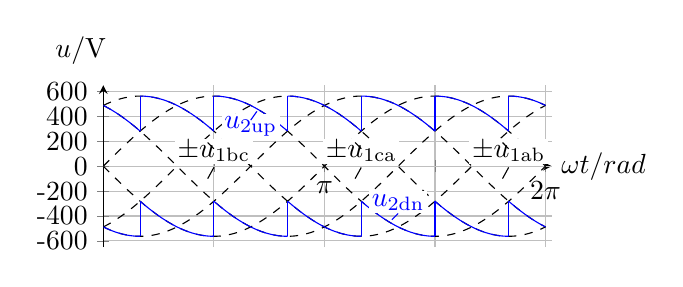
\begin{tikzpicture}
            \begin{axis}[
                % x/y range adjustment
                xmin=0, xmax=365,
                ymin=-650, ymax=650,
                samples=500,
                axis y line=center,
                axis x line=middle,
                extra y ticks=0,
                % Label text
                xlabel={$\omega t / \text{rad}$},,
                ylabel={$u/\mathrm{V}$},
                % Label adjustment
                x label style={at={(axis description cs:1,0.5)},anchor=west},
                y label style={at={(axis description cs:-.05,.97)},anchor=south,yshift=0.2cm},
                width=0.6\textwidth,
                height=0.3\textwidth,
                % x-Ticks
                xtick={0,90,180,270,360},
                xticklabels={,,$\pi$,,$2\pi$},
                xticklabel style = {anchor=north},
                % y-Ticks
                ytick={600,400,200,0,-200,-400,-600},
                yticklabels={600,400,200,0,-200,-400,-600},
                yticklabel style = {anchor=east},
                % Grid layout
                grid,
                %grid style={line width=.1pt, draw=gray!10},
                %major grid style={line width=.2pt,draw=gray!90},
            ]
            % Voltage u1ab(wt), u1bc(wt) u1ca(wt)
            \addplot[black, domain= 0:360,dashed] {563*cos(x-30)};                
            \addplot[black, domain= 0:360,dashed] {563*cos(x+90)};                
            \addplot[black, domain= 0:360,dashed] {563*cos(x+210)}; 
            % Voltage -u1ab(wt), -u1bc(wt) -u1ca(wt)
            \addplot[black, domain= 0:360,dashed] {-563*cos(x-30)};                
            \addplot[black, domain= 0:360,dashed] {-563*cos(x+90)};                
            \addplot[black, domain= 0:360,dashed] {-563*cos(x+210)}; 
            % Voltage u2(wt) up
            \addplot[blue, domain= 0:30] {-563*cos(x+210)};            
            \addplot[blue, domain= 30:90] {563*cos(x-30)};                
            \addplot[blue, domain= 270:330] {563*cos(x+90)};                
            \addplot[blue, domain= 150:210] {563*cos(x+210)}; 
            \addplot[blue, domain= 210:270] {-563*cos(x-30)};                
            \addplot[blue, domain= 90:150] {-563*cos(x+90)};                
            \addplot[blue, domain= 330:360] {-563*cos(x+210)};            
            \addplot[color=blue,solid] coordinates{
                (30, 563)
                (30, 282)
            };     
            \addplot[color=blue,solid] coordinates{
                (90, 563)
                (90, 282)
            };     
            \addplot[color=blue,solid] coordinates{
                (150, 563)
                (150, 282)
            };     
            \addplot[color=blue,solid] coordinates{
                (210, 563)
                (210, 282)
            };     
            \addplot[color=blue,solid] coordinates{
                (270, 563)
                (270, 282)
            };     
            \addplot[color=blue,solid] coordinates{
                (330, 563)
                (330, 282)
            };     
    
            % Voltage u2(wt) down
            \addplot[blue, domain= 0:30] {-563*cos(x-30)};                
            \addplot[blue, domain= 150:210] {563*cos(x-30)};                
            \addplot[blue, domain= 30:90] {563*cos(x+90)};                
            \addplot[blue, domain= 270:330] {563*cos(x+210)};            
            \addplot[blue, domain= 330:360] {-563*cos(x-30)};                
            \addplot[blue, domain= 210:270] {-563*cos(x+90)};                
            \addplot[blue, domain= 90:150] {-563*cos(x+210)}; 
            \addplot[color=blue,solid] coordinates{
                (30,-563)
                (30,-282)
            };     
            \addplot[color=blue,solid] coordinates{
                (90,-563)
                (90,-282)
            };     
            \addplot[color=blue,solid] coordinates{
                (150,-563)
                (150,-282)
            };     
            \addplot[color=blue,solid] coordinates{
                (210,-563)
                (210,-282)
            };     
            \addplot[color=blue,solid] coordinates{
                (270,-563)
                (270,-282)
            };     
            \addplot[color=blue,solid] coordinates{
                (330,-563)
                (330,-282)
            };     
         
            % Label of +-u1bc
            \node[black, fill=white, inner sep = 1pt, anchor = south] at (axis cs:90,10) {$\pm u_{\mathrm{1bc}}$};
            % Line to +u1bc
            \draw[thin, black] (90,140) -- (85,190);            
            % Line to -u1bc
            \draw[thin, black] (90,-10) -- (85,-100);            
            % Label of +-u1ca
            \node[black, fill=white, inner sep = 1pt, anchor = south] at (axis cs:210,10) {$\pm u_{\mathrm{1ca}}$};
            % Line to +u1ca
            \draw[thin, black] (210,140) -- (205,190);            
            % Line to -u1ca
            \draw[thin, black] (210,-10) -- (205,-100);   
            % Label of +-u1ab
            \node[black, fill=white, inner sep = 1pt, anchor = south] at (axis cs:330,10) {$\pm u_{\mathrm{1ab}}$};
            % Line to +u1ab
            \draw[thin, black] (330,140) -- (325,190);            
            % Line to -u1ab
            \draw[thin, black] (330,-10) -- (325,-100);               
            % Label of u2up
            \node[blue, fill=white, inner sep = 1pt, anchor = south] at (axis cs:120,210) {$u_{\mathrm{2 up}}$};
            % Line to u2,p
            \draw[thin, blue] (120,370) -- (125,440);
            % Label of u2,m
            \node[blue, fill=white, inner sep = 1pt, anchor = south] at (axis cs:240,-380) {$u_{\mathrm{2 dn}}$};
            % Line to u2,m
            \draw[thin, blue] (240,-380) -- (235,-430);
        \end{axis}     
        \end{tikzpicture}
        \caption{Output voltage $u_\mathrm{2 up}(\omega t)$ for raising and $u_\mathrm{2 dn}(\omega t)$ lowing load.}
        \label{sfig:ex06_Voltage_u2pmn_down}
\end{solutionfigure}